\documentclass{article}
\usepackage[utf8]{inputenc}
\usepackage{graphicx}

\title{Laporan Database}
\author{itsmeakil707 }
\date{October 2019}

\begin{document}

\title{Laporan Database}
\author{Akil Munawwar \\ 1184041 \\ D4 TI 1B}
\maketitle

\part{Rangkuman Video}
\paragraph{}
Dari video yang saya saksikan saat live streaming kemarin. Saya memahami beberapa hal, yaitu apa itu oracle apex, dan bagaimana cara membuat suatu workspace pada oracle apex.
\section{Pengertian Oracle Apex}
\paragraph{}
Oracle Application Express (APEX) adalah suatu platform yang digunakan untuk membangun aplikasi yang aman, dengan fitur kelas dunia dan dapat digunakan dimana saja. Dalam APEX ini terdapat tiga alat utama yang digunakan.
\begin{enumerate}
    \item Application Builder
    \paragraph{} Membuat aplikasi, melihat aplikasi, mengimport aplikasi, mengatur service, mengatur user aplikasi dan memantau aktifitas yang di lakukan pengguna.
    \item SQL Workshop
    \paragraph{} Membuat tabel dan komponennya (menggunakan kode PL-SQL secara manual maupun otomatis), melihat struktur tabel dan komponennya, mengimpor dan mengekspor script.
    \item Utility
    \paragraph{} Melihat report table dan komponennya dan history aplikasi.
\end{enumerate}
\newpage

\section{Cara membuat Workspace di APEX} 
\begin{enumerate}
    \item Pertama pastikan anda sudah menginstall APEX pada komputer atau laptop anda.
    \item Kedua, buka http://127.0.0.1:8080/apex/f?p=4550:10:10960410872195:::::
    \begin{figure}[!htbp]
        \centering
        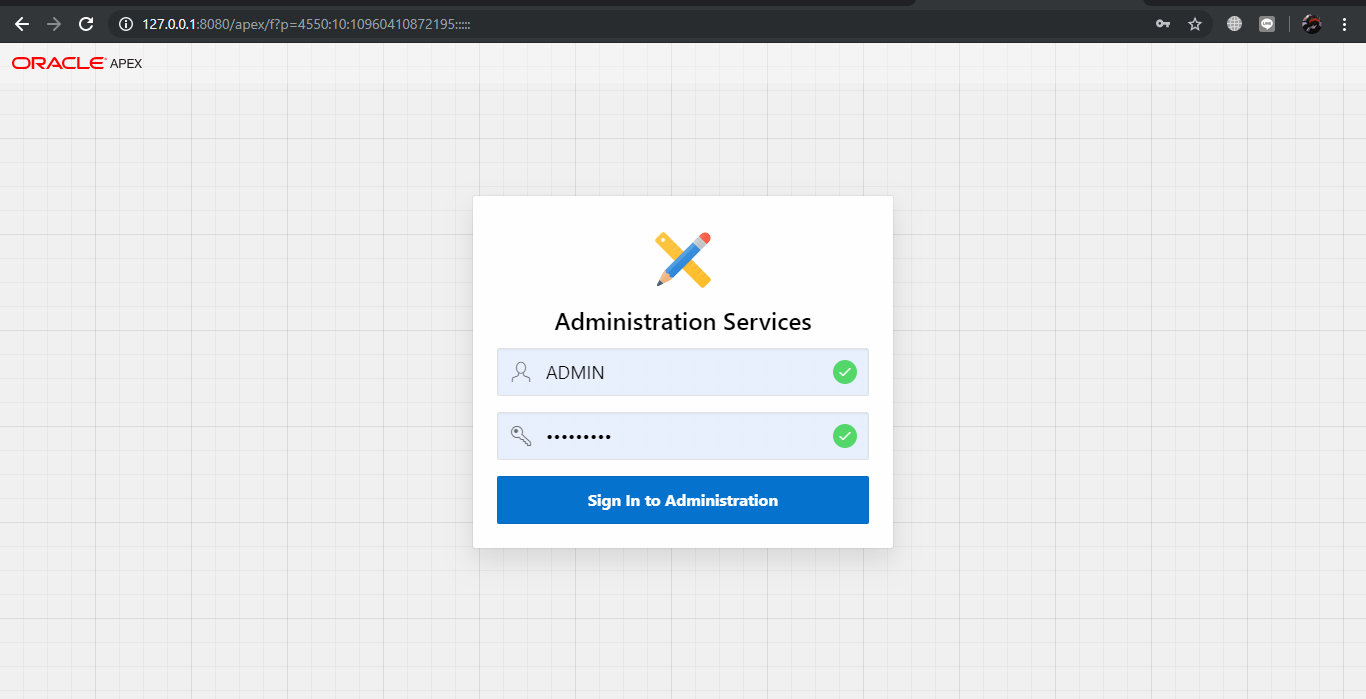
\includegraphics[scale=0.3]{LangkahPertama.PNG}
        \caption{Hal Utama Login}
    \end{figure}
    \item Setelah itu, login dengan akun yang sudah kalian buat waktu install APEX tersebut.
    \item Jika sudah, maka akan masuk ke halaman utama.
    \item Setelah itu klik \textit{Create Workspace}
    \begin{figure}[!htbp]
        \centering
        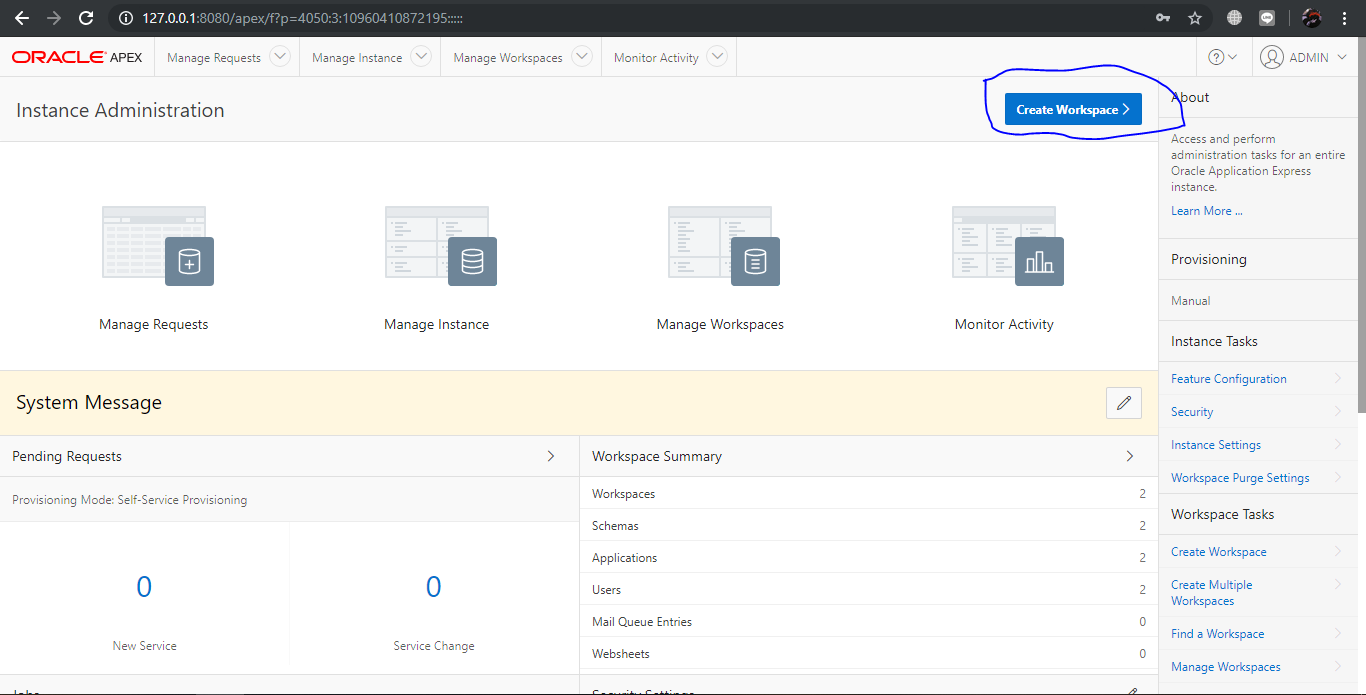
\includegraphics[scale=0.3]{LangkahKedua.PNG}
        \caption{Halaman Utama}
    \end{figure}
\newpage
    \item Setelah itu, buat nama dari workspace nya, sisanya kalian boleh kosongkan dan itu tidak akan berpengaruh.
    \begin{figure}[!htbp]
        \centering
        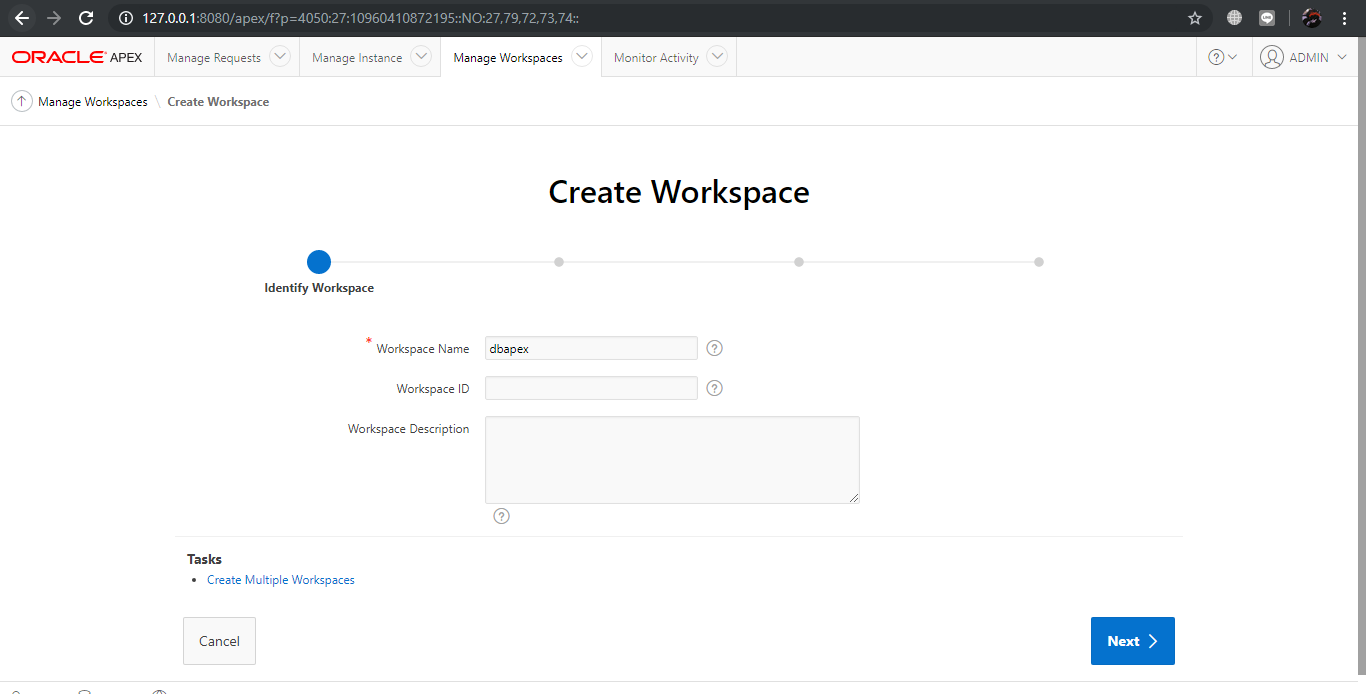
\includegraphics[scale=0.3]{LangkahKetiga.PNG}
        \caption{Pemberian Nama Workspace}
    \end{figure}
    \item Setelah itu, klik next
    \item Langkah selanjutnya, buat pengaturan seperti gambar dibawah ini.
    \begin{figure}[!htbp]
        \centering
        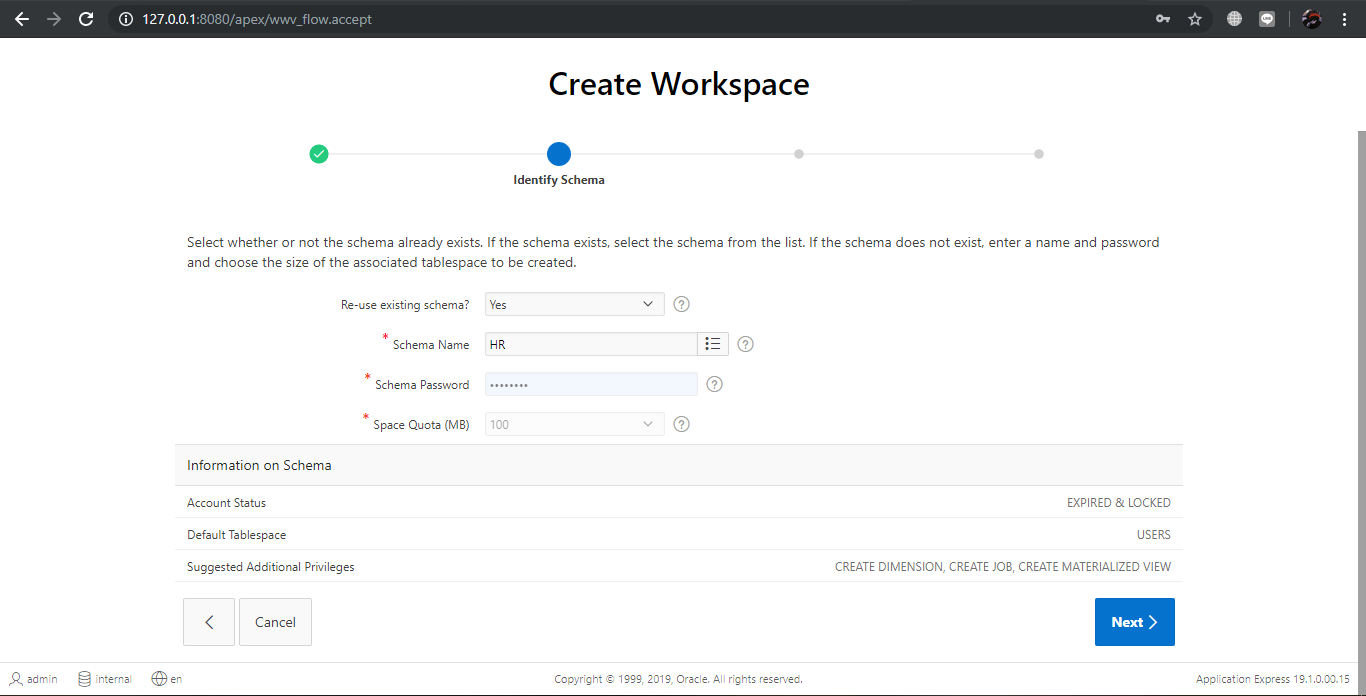
\includegraphics[scale=0.3]{LangkahKeempat.PNG}
        \caption{Pengaturan Pada Skema}
    \end{figure}
    \item Untuk mengubah skema nya menjadi HR, maka klik di samping ADMIN, nanti akan ada pop up berisi HR.
\newpage
    \item Setelah itu klik next.
    \item Setelah next, maka akan ada tampilan seperti ini.
    \begin{figure}[!htbp]
        \centering
        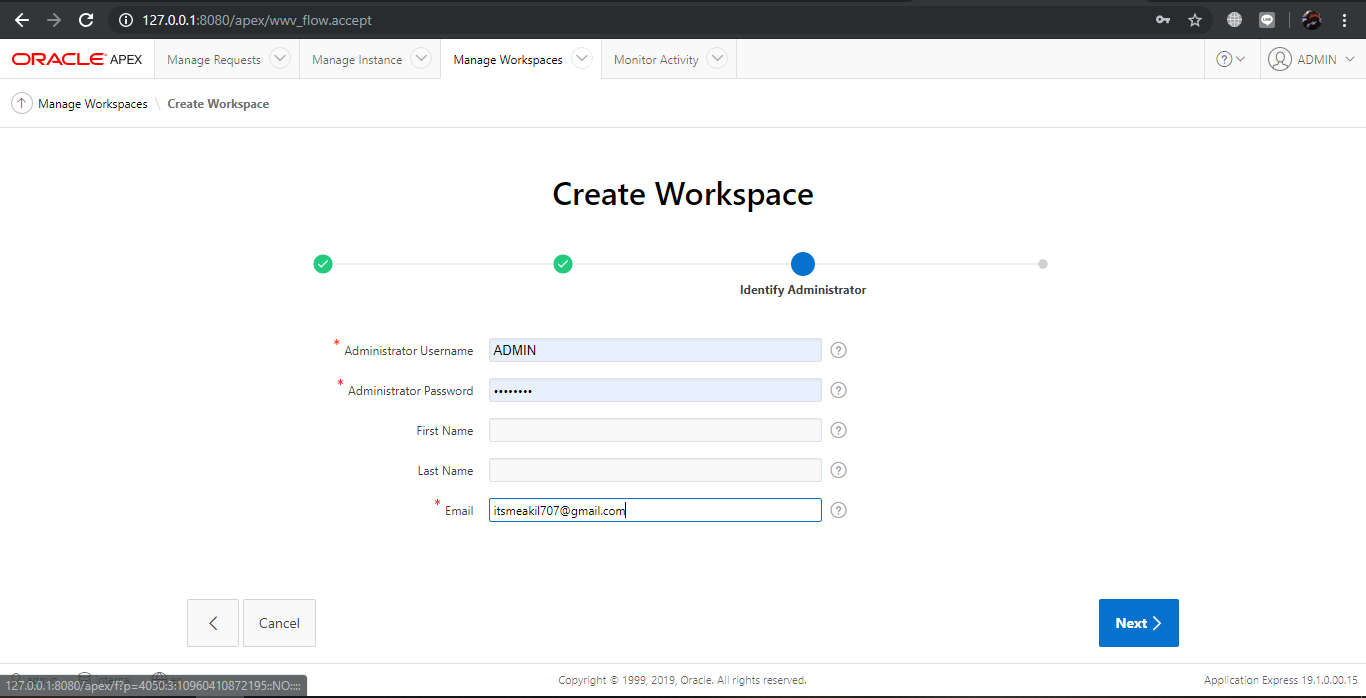
\includegraphics[scale=0.3]{LangkahKelima.PNG}
        \caption{Pengaturan Administrator}
    \end{figure}
    \item Nantinya, akan mengatur nama username dan password untuk login nantinya.
    \item Setelah itu, atur email dengan email kalian. Untuk first dan last name bisa dikosongkan.
    \item Klik next
    \item Setelah next, akan ada konfirmasi kembali mengenai workspace.
    \begin{figure}[!htbp]
        \centering
        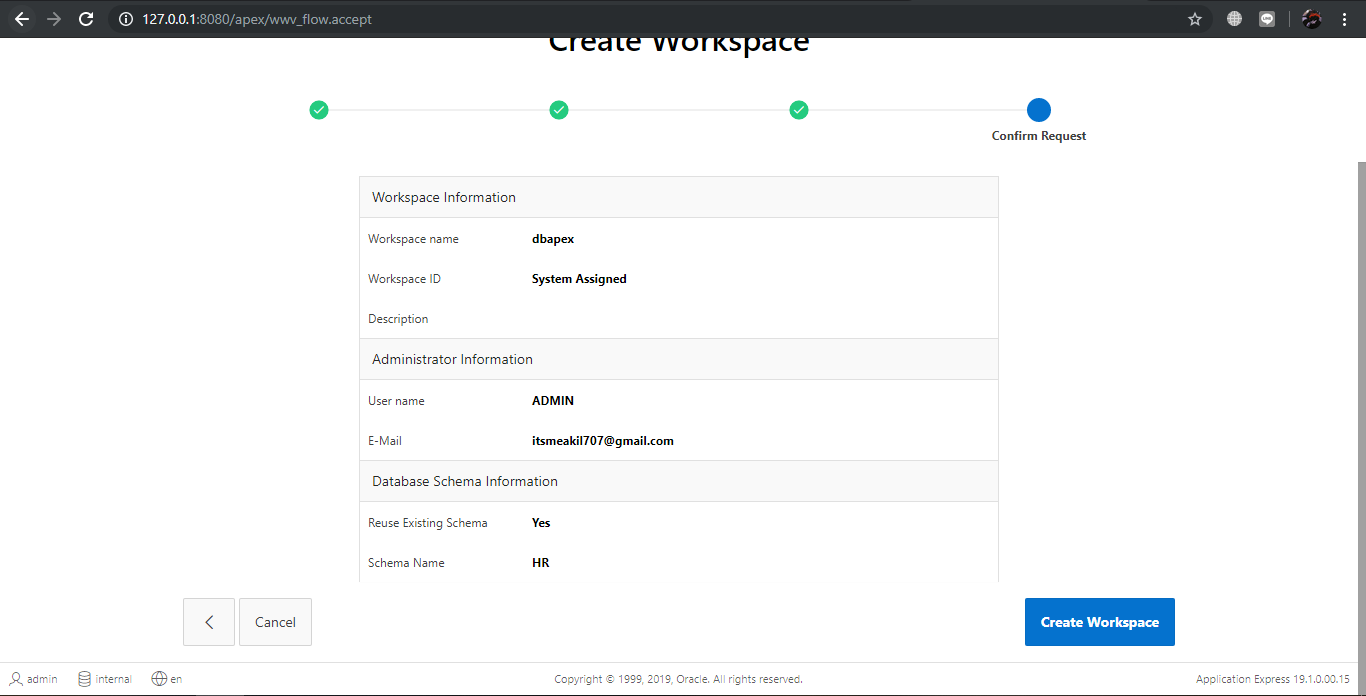
\includegraphics[scale=0.3]{LangkahKeenam.PNG}
        \caption{Konfirmasi Workspace}
    \end{figure}
    \item Jika sudah maka klik create workspace
\newpage
    \item Jika sudah berhasil, maka selanjutnya pergi ke http://127.0.0.1:8080/apex/f?p=4550:1:12275980854321:::::
    \item Maka Login sesuai dengan nama workspace dan username password tadi.
    \begin{figure}[!htbp]
        \centering
        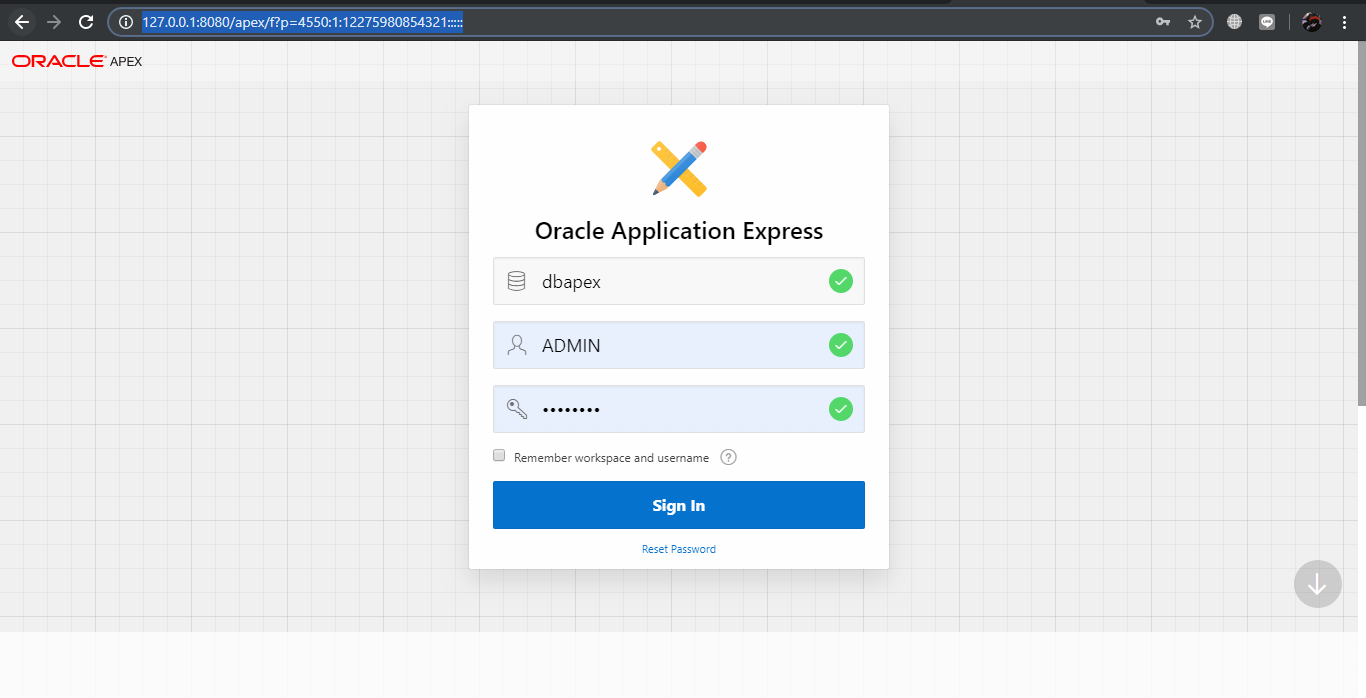
\includegraphics[scale=0.3]{LangkahKetujuh.PNG}
        \caption{Login Workspace}
    \end{figure}
    \item Setelah login, maka akan ada disuruh ubah password.
    \begin{figure}[!htbp]
        \centering
        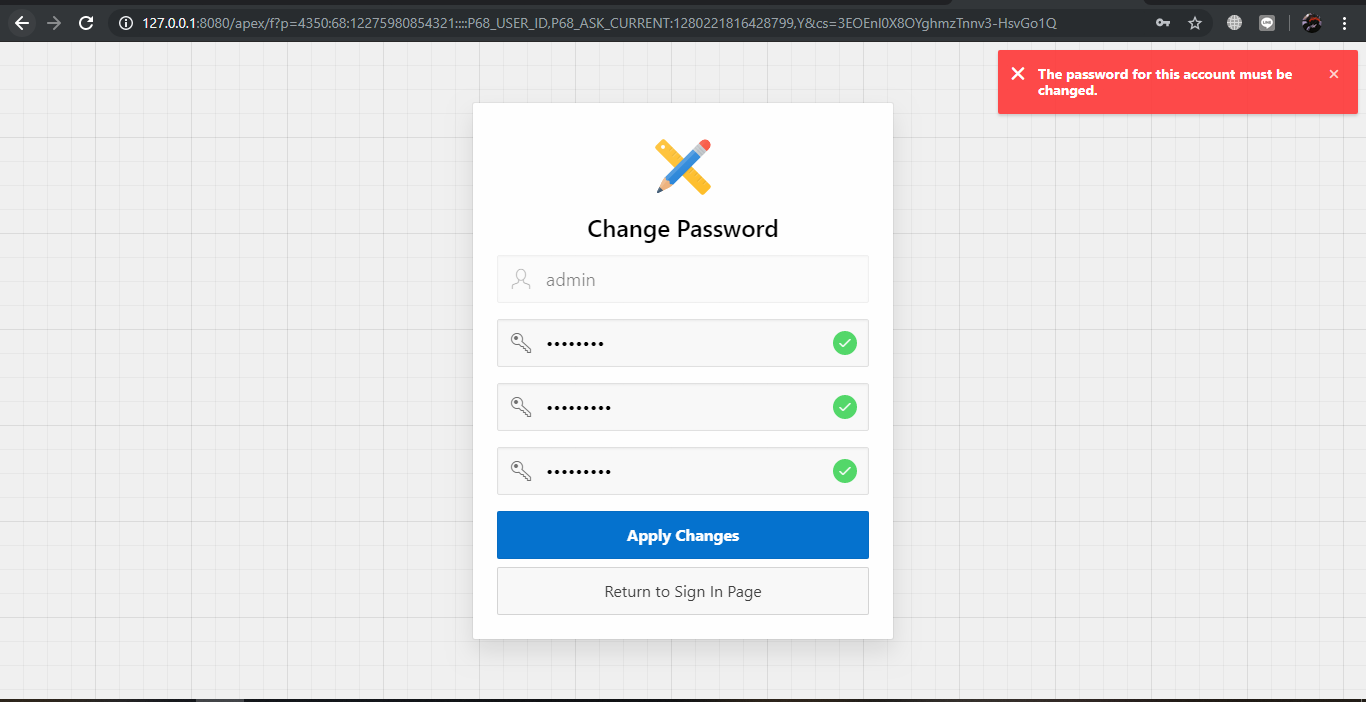
\includegraphics[scale=0.3]{LangkahKedelapan.PNG}
        \caption{Hal Ubah Password}
    \end{figure}
\newpage
    \item Jika sudah selesai, maka akan langsung menuju hal workspace
    \begin{figure}[!htbp]
        \centering
        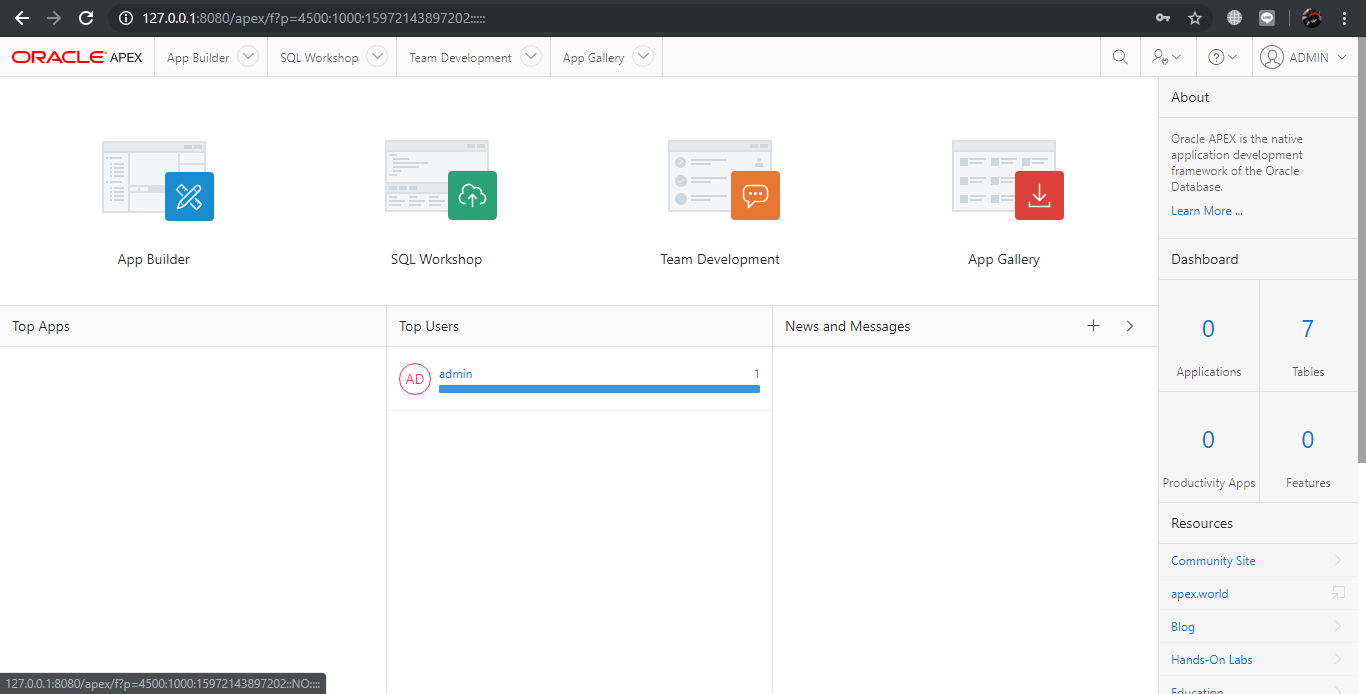
\includegraphics[scale=0.3]{LangkahTerakhir.PNG}
        \caption{Hal Workspace}
    \end{figure}
\end{enumerate}
\end{document}
